\section{Dynamic model} \label{sec:dynamic_model}

\subsection{Single joint model} \label{Single joint model}
%\hldone{DONE}
The joints of the exoskeleton can be modeled with a lumped parameter model due to the elasticity of the harmonic drive speed reducer and torque sensor (for joints 1, 2 and 4) and of tendon transmission for joint 3. The used single joint model is a 2-mass with spring and damper (Fig. \ref{fig:exos_singlejoint_model}).

\par The single joint dynamics is formulated by the following equations:

\setlength{\arraycolsep}{0.0em}
\footnotesize
\begin{align}
%\label{eqn:dinamicaMotoreSingoloGiunto}
I_{m,i} \ddot{\theta}_{m,i}  + c_{m,i}\dot{\theta}_{m,i} + c_{t,i} (\dot{\theta}_{m,i}-\dot{\theta}_{i})  
{+}\:k_{t,i} ({\theta_{m,i}}-{\theta_i}) &= \tau_{m,i}+\tau_ {d,i} \nonumber	\\
\label{eqn:dinamicaLinkSingoloGiunto}
I_{l,i} \ddot{\theta}_{i}+c_{t,i} (\dot{\theta}_{i}-\dot{\theta}_{m,i})
+k_{t,i} ({\theta_{i}}-{\theta_{m,i}}) &= \tau_{l,i}	
\end{align}
\normalsize
\setlength{\arraycolsep}{5pt}

where referring to the i-th joint, $\theta_ {m,i}$ and $\theta_ {i}$ stand for motor and joint angles respectively, $k_{t,i}$ and $c_{t,i}$ are the stiffness and viscous coefficient of the transmission, that were experimentally characterized.
$I_{m,i}$ is motor inertia, $I_{l,i}$ is average link inertia considered as constant, $\tau_{m,i}$ is the motor torque, $\tau_{d,i}$ is a disturbance torque acting on the motor rotor  which accounts for internal friction and ripple effects of both motor and harmonic drive, while $\tau_{l,i}$ is the external torque acting directly on the output link. The $\tau_{l,i}$ torque accounts for the 
exogenous input due to the interaction  with the human, and endogenous input accounting for unmodeled non-linear effects, such as dynamic or gravity forces.
\begin{figure}[ht]
	\centering
	%{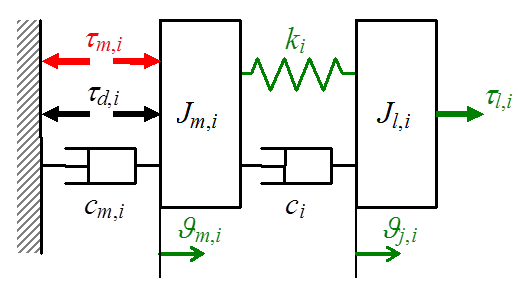
\includegraphics[width=0.5\columnwidth]{2massModel}}
	\def\svgwidth{0.7\columnwidth}
	\begin{footnotesize}
		\input{imgRevised/2MassModel.pdf_tex}
	\end{footnotesize}
	\caption{The 2-mass model for each joint.}
	\label{fig:exos_singlejoint_model}
\end{figure}
%%%%%%%%%%%%%%%%%%%%%%%%%%%%%%%%%%%%%%%%%%%%%%%%%%%%%%%%%%%%%%%%%%%%%%%%%%%%%%%%%%%%%%%%%%%%%%%%%%%%%%%%%%%%%%%%%%%%
%%%%%%%%%%%%%%%%%%%%%%%%%%%%%%%%%%%%%%%%%%%%%%%%%%%%%%%%%%%%%%%%%%%%%%%%%%%%%%%%%%%%%%%%%%%%%%%%%%%%%%%%%%%%%%%%%%%%
\subsubsection{Experimental characterization of single joint performance}
%\hldone{DONE}
%\point{Insert here experimental data and procedures with indication of dynamic bandwidth}
As described in \ref{subsec:mechanicalDesign} the joint is equipped with a torque sensor that is a part of the transmission chain and is capable of measuring the elastic torque $\tau_{s,i}$, which acts between motor rotor and joint output link. The elastic sensor torque can be expressed by $\tau_{s,i} = k_{t,i} (\theta_{i}-\theta_{m,i})$. The joint dynamics can be re-written expliciting the $\tau_{s,i}$ readings starting from  $\tau_{s,i}$ definition, its 1st and 2nd derivatives and using the equations  \ref{eqn:dinamicaLinkSingoloGiunto}. It is obtained:
\begin{equation}
\label{eqn:dinamicaSensoreCoppia}
\ddot{\tau}_{s,i} + \frac{c_{t,i}}{I_i}\dot{\tau}_{s,i} + \frac{k_{t,i}}{I_i}\tau_{s,i}= \frac{k_{t,i}}{I_{l,i}}\tau_l + \frac{k_{t,i}}{I_{l,i}}\tau_g - \frac{k_{t,i}}{I_{m,i}}\tau_d - \frac{k_{t,i}}{I_{m,i}}\tau_m
\end{equation}
where $I_i = I_l I_m /(I_l+I_m)$. The natural frequency of this system is $\omega_n = \sqrt{k_{t,i} /I_i } /2\pi$. The natural frequency has been experimentally evaluated for a single joint in a test-rig analyzing the response of the $\tau_s$ when a chirp command is used for the $\tau_m$ motor torque. 
\par From Fig. \ref{fig:OpenLoopJointBode}, use of the Half-Power Bandwidth method returns $c = 11.8 \, \text{Nms/rad}$ as the overall damping coefficient of the flexible joint (this value has also been validated via the Logarithmic Decrement method).
\begin{figure}[ht]
	\centering
%	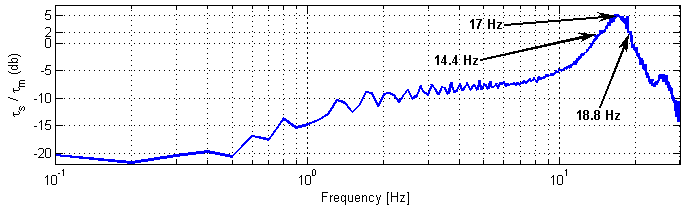
\includegraphics[width=1\columnwidth]{OpenLoopJointBode}
	\def\svgwidth{1\columnwidth}
	\begin{footnotesize}
		\input{imgRevised/bode_rehab_joint.pdf_tex}
	\end{footnotesize}
	\caption{Experimental open-loop response (Bode magnitude plot) of joints 1,2 and 4: joint sensor torque vs. motor torque command in standardized testbed conditions.}
	\label{fig:OpenLoopJointBode}
\end{figure}
Considering the exoskeleton, every joint sees a link inertia that depends on the pose so the natural frequency of each joint depends on the pose of the exoskeleton. 
Considering an average link inertia, it can be obtained the natural frequency for each joint elastic transmission. Results are shown in the \tablename \ \ref{tab:naturalFrequencies}.
%\begin{table}[!t]
%	\renewcommand{\arraystretch}{1.3}
%	\caption{The natural frequency of the joints}
%	\label{tab:naturalFrequencies}
%	\centering
%	\begin{tabular}{|c|c|c|}
%		\hline
%		\bfseries Joint & \bfseries Avg. link inertia [$Kg/m^2$] & \bfseries Natural freq. [$Hz$]\\
%		\hline\hline
%		1 & 0.9639 & 19.3930\\
%		\hline
%		2 & 1.11 & 18.3501\\
%		\hline
%		4 & 0.1925 & 39.6797\\
%		\hline
%	\end{tabular}
%\end{table}
\begin{table}[!t]
	\renewcommand{\arraystretch}{1.3}
	\caption{The natural frequency of the joints}
	\label{tab:naturalFrequencies}
	\centering
	\begin{tabular}{c c c}
		\hline \hline
		\bfseries Joint & \bfseries Avg. link inertia [$Kg/m^2$] & \bfseries Natural freq. [$Hz$]\\
		\hline
		1 & 0.9639 & 19.3930\\
		2 & 1.11 & 18.3501\\
		4 & 0.1925 & 39.6797\\
		\hline \hline
	\end{tabular}
\end{table}
For all these three joints the motor inertia is the same and it is equivalent to $3.742 \, \text{ Kg/m}^2$.


%%%%%%%%%%%%%%%%%%%%%%%%%%%%%%%%%%%%%%%%%%%%%%%%%%%%%%%%%%%%%%%%%%%%%%%%%%%%%%%%%%%%%%%%%%%%%%%%%%%%%%%%%%%%%%%%%%%%
%%%%%%%%%%%%%%%%%%%%%%%%%%%%%%%%%%%%%%%%%%%%%%%%%%%%%%%%%%%%%%%%%%%%%%%%%%%%%%%%%%%%%%%%%%%%%%%%%%%%%%%%%%%%%%%%%%%%
%%%%%%%%%%%%%%%%%%%%%%%%%%%%%%%%%%%%%%%%%%%%%%%%%%%%%%%%%%%%%%%%%%%%%%%%%%%%%%%%%%%%%%%%%%%%%%%%%%%%%%%%%%%%%%%%%%%%
%%%%%%%%%%%%%%%%%%%%%%%%%%%%%%%%%%%%%%%%%%%%%%%%%%%%%%%%%%%%%%%%%%%%%%%%%%%%%%%%%%%%%%%%%%%%%%%%%%%%%%%%%%%%%%%%%%%%
\subsection{Multiple joints model} \label{Full dynamics model}

Given the single joint two-mass model, the dynamic model of the whole exoskeleton can be formulated in matrix form as follows:
\setlength{\arraycolsep}{0.0em}


%\footnotesize

\begin{equation}
%\left \{
\begin{IEEEeqnarraybox}[][c]{l}
\overbrace{\colorboxed{red}{\vectm{I_m}    \vectm{D} \vects{\ddot{\uptheta}_m} + \vectm{B_m } \vectm{D} \vects{\dot{\uptheta}_m} }}^{\text{Motor Dynamics}}
 +
  \overbrace{  \colorboxed{green}{\vectm{C_t}  ( \vectm{D} \vects{\dot{\uptheta}_m} - \vects{\dot{\uptheta}} )+ 
  		\:\vectm{K_t}  ( \vectm{D} \vects{\uptheta_m}- \vects{\uptheta} ) }}^{\text{Elastic transmission torque}}
  =  \\ \vects{\uptau_m} +\vects{\uptau_d}   \\
\underbrace{\colorboxed{red}{\vectm{M}(\vects{\uptheta}) \vects{\ddot{\uptheta}}  + \vectm{C}( \vects{\dot{\uptheta}}, \vects{\uptheta})   \vects{\dot{\uptheta}}}}_{\text{Joint dynamics}}
 +   
 %\underbrace{  \colorboxed{green}{ }}_{\text{Joint dynamics}}
\underbrace{  \colorboxed{green}{
 \vectm{C_t}  ( \vects{\dot{\uptheta}} - \vectm{D} \vects{ \dot{\uptheta}_m} )
{+}\: \vectm{K_t}  ( \vects{\uptheta} - \vectm{D}\vects{\uptheta_m} )}}_{\text{Elastic transmission torque}} + \\ + \vect{G}( \vects{\uptheta}) = \vectm{J^T} \vect{F_h}
\label{eqn:dinamicaLinkMultiGiunto}
\end{IEEEeqnarraybox}
%\right . %\label{eqn:dinamicaMotoreMultiGiunto}
\end{equation}
%\label{eqn:dinamicaMotoreMultiGiunto} 
\normalsize
\setlength{\arraycolsep}{5pt}
%
%\fbox{$\displaystyle
%	\smash{\callout{F}{\stackunder{$1,n$}{we only consider 1 unknown}}} = 
%	\left[
%	\frac{\partial f}{\partial l_1}\quad
%	\frac{\partial f}{\partial l_2}\quad
%	\frac{\partial f}{\partial l_3}
%	\cdots
%	\frac{\partial f}{\partial l_n}
%	\right]
%	$}
%
%\vspace{2 cm }

%\begin{eqnarray}
%\label{eqn:dinamicaMotoreMultiGiunto}
%\vectm{J_m}    \vectm{D} \vects{\ddot{\theta}_m} + \vectm{B_m  D} \vects{\dot{\theta}_m}  + \vectm{C_t}  ( \vectm{D} \vects{\dot{\theta}_m} - \vects{\dot{\theta}_j} )+ 
%\:\vectm{K_t}  ( \vectm{D} \vects{\theta_m}- \vects{\theta_j} ) =  \nonumber\\ \vects{\tau_m} +\vects{\tau_d}
%\end{eqnarray}


%\begin{eqnarray}
%\label{eqn:dinamicaLinkMultiGiunto}
%\vectm{M}(\vects{\theta_j}) \vects{\ddot{\theta}_j}  + \vectm{C}( \vects{\dot{\theta}_j}, \vects{\theta_j})   \vects{\dot{\theta}_j} +   \vectm{C_t}  ( \vects{\dot{\theta}_j} - \vectm{D} \vects{ \dot{\theta}_m} )+ 
%{+}\: \vectm{K_t}  ( \vects{\theta_j} - \vectm{D}\vects{\theta_m} ) + \nonumber\\ + \vects{G}( \vects{\theta_j}) = \vectm{J}^T \vects{F_h}
%\end{eqnarray}


%where $\vectm{D}$ is a diagonal matrix modeling the reduction factor introduced by joint speed reducers, $\vectm{J_m}$ and $\vectm{B_m}$ are diagonal matrices modeling inertia and viscous friction at motor respectively; $\vectm{K_t}$ and $\vectm{C_t}$ are diagonal matrices modeling stiffness and damping associated to the elastic transmission; $\vects{G}$ models the effects of gravity force on links.
where $\vectm{I_m}$, $\vectm{B_m}$, $\vectm{D}$, $\vectm{K_t}$ and $\vectm{C_t}$ are diagonal matrices.  $\vectm{I_m}$ and $\vectm{B_m}$ model inertia and viscous friction at motor respectively, while $\vectm{K_t}$ and $\vectm{C_t}$ model stiffness and damping associated with the elastic transmission and $\vectm{D}$ models  the transmission reduction factor introduced by joint gearheads; $\vect{G}$ models the effects of gravity force on links;
$\vect{F_h}$ are the external  forces  acting on the system  due to human interaction  and the respective joint torques are computed by multiplying them by the transposed Jacobian matrix  $\vectm{J^T}$ evaluated in the actual exoskeleton configuration. The multi-joint model introduces cross-coupling among joints and non-linearities, with terms $ \vectm{C}( \vects{\dot{\uptheta}}, \vects{\uptheta})  $ that models Coriolis effects and $\vectm{M}(\vects{\uptheta}) $ that represents link inertias and that can be decomposed
into a diagonal constant component and a variable component as follows:

%By taking into account that
%that the real dynamics has terms  $\vectm{M}(\vects{\uptheta}) $  and $ \vectm{C}( \vects{\dot{\uptheta}}, \vects{\uptheta}) $ depending on the actual joint configuration, the first term can be decoupled into a diagonal constant component and a variable component as follows:
\begin{equation}
\vectm{M }  \vects{\ddot{\uptheta}}=
\underbrace{\overline{\vectm{M} } \vects{\ddot{\uptheta}}}_{\text{constant}}
 + 
\underbrace{\vects{\Delta} \vectm{M} (\vects{\uptheta}) \vects{\ddot{\uptheta}} }_{\text{variable}}
\label{eq:InertialComponent}
\end{equation}
By making a replacement of variables introducing this expression for the  joint torque 
\begin{equation} 
\vects{\uptau_s}=-\vectm{K_t}  ( \vectm{D} \vects{\uptheta_m}- \vects{\uptheta} ) \label{eq:taus} 
\end{equation}
the dynamics equations (\ref{eqn:dinamicaLinkMultiGiunto}) can be reformulated as follows in terms of new variables $\vects{\uptau_s}$ and $\vects{\uptheta_m}$:
%\footnotesize
%\begin{equation}
%\left \{
%\begin{aligned}
%\vects{\tau_s} & = - \vectm{K_t}  ( \vectm{D} \vects{\uptheta_m}- \vects{\uptheta} ) \\
%\vects{\dot{\tau_s}} & = - \vectm{K_t}  ( \vectm{D}  \vects{\dot{\uptheta}_m} - \vects{\dot{\uptheta}} ) \\
%\vects{\ddot{\tau_s}} & = - \vectm{K_t}  ( \vectm{D}  \vects{\ddot{\uptheta}_m} - \vects{\ddot{\uptheta}} ) \\
%\end{aligned}
%\right .
%\label{eq:taus}
%\end{equation}
%\normalsize


%\footnotesize
\begin{equation}
\boxed{
\left
 \{
\begin{IEEEeqnarraybox}[][c]{l}
\vectm{ I_m  D } \vects{ \ddot{\uptheta}_m} + \vectm{B_m D}\vects{\dot{\uptheta}_m}  = \vectm{K_t}^{-1} \vectm{C_t}\vects{ \dot{\uptau}_s} + \vects{\uptau_s} +\vects{\uptau_d} + \vect{u} \\ 
\vects{\ddot{\uptau}_s}  + \vectm{C_t I_i}^{-1} \vects{\dot{\uptau}_s} + \vectm{K_t I_i}^{-1} \vects{\tau_s}= \vectm{K_t I_{m}}^{-1} (\vectm{I_{m}} \overline{\vectm{M}}^{-1}  \vectm{J}^T \vects{F_l}  +  \\
{+}\:  \vectm{B_m D}\vects{\dot{\uptheta}_m}-\vects{\uptau_d} - \vect{u})
\end{IEEEeqnarraybox}
\right .
}
\label{eq:dynEqRewritten}
\end{equation}
\normalsize
%\label{eq:dynamics_eq1}
%\label{eq:dynamics_eq2}
\setlength{\arraycolsep}{0.0em}



%%%COPY MADE BY ANTONIO BEFOREMODIFYING
%
%
%%\footnotesize
%\begin{equation}
%\boxed{
%	\left
%	\{
%	\begin{IEEEeqnarraybox}[][c]{l}
%	\vectm{ I_m  D } \vects{ \ddot{\uptheta}_m} + \vectm{B_m D}\vects{\dot{\uptheta}_m}  = \vectm{K_t}^{-1} \vectm{C_t}\vects{ \dot{\uptau}_s} + \vects{\uptau_s} +\vects{\uptau_d} + \vect{u} \\ 
%	\vects{\ddot{\uptau}_s}  + \vectm{C_t I_i}^{-1} \vects{\dot{\uptau}_s} + \vectm{K_t I_i}^{-1} \vects{\tau_s}= \vectm{K_t   I_m}^{-1}  \vectm{B_m D}\vects{\dot{\uptheta}_m}+  \\
%	{+}\:\overline{\vectm{M}}^{-1} \vectm{K_t J}^T \vects{F_l} - \vectm{K_t I_{m}}^{-1} (\vects{\uptau_d} + \vect{u})
%	\end{IEEEeqnarraybox}
%	\right .
%}
%\label{eq:taus}
%\end{equation}
%\normalsize
%%\label{eq:dynamics_eq1}
%%\label{eq:dynamics_eq2}
%\setlength{\arraycolsep}{0.0em}

\setlength{\arraycolsep}{5pt}

where  $\vect{u}$ (see appendix) represents the actual control command and the external  disturbance forces  have been collected within the external load  force  $\vects{F_l}$  term (see Appendix I for detailed derivation of terms).

This form of the dynamics equation is useful for defining a full-state feedback control law and an optimal observer for the estimation of joint torque.

%\begin{multline}
%%\begin{aligned}
% \overline{M}K_t^{-1}\vects{\ddot{\tau_s}} + K_t^{-1}  C_t (I+  \overline{M} J_m^{-1}) ]\vects{\dot{\tau_s}}  +\\
% + (I+   \overline{M} J_m^{-1})\vects{\tau_s}  =  \overline{M}(\vects{q_j}) J_m^{-1}  B_m    D  \dot{\vects{\theta}}_m   \\ +  J^T  \vects{F_{l}}-\overline{M} J_m^{-1} \vects{u}- \overline{M} J_{m}^{-1}\vects{\tau_d}
%%\end{aligned}
%\label{eqdyn}
%\end{multline}


%so if 
%then it follows that 
%$$[I+  \overline{M} J_m^{-1}]=\overline{M} J_i^{-1}$$
%then by replacing $J_i$ in equation 	\eqref{eqdyn}, we find the  set of dynamic equations: 



%%%%%%%%%%%%%%%%%%%%%%%%%%%%%%%%%%%%%%%%%%%%%%%%%%%%%%%%%%%%%%%%%%%%%%%%%%%%%%%%%%%%%%%%%%%%%%%%%%%%%%%%%%%%%%%%%%%%
%%%%%%%%%%%%%%%%%%%%%%%%%%%%%%%%%%%%%%%%%%%%%%%%%%%%%%%%%%%%%%%%%%%%%%%%%%%%%%%%%%%%%%%%%%%%%%%%%%%%%%%%%%%%%%%%%%%%
%\subsection{(?) Different models for interaction torque control}
%
%\label{Centralized interaction torque control}

%%%%%%%%%%%%%%%%%%%%%%%%%%%%%%%%%%%%%%%%%%%%%%%%%%%%%%%%%%%%%%%%%%%%%%%%%%%%%%%%%%%%%%%%%%%%%%%%%%%%%%%%%%%%%%%%%%%%
%%%%%%%%%%%%%%%%%%%%%%%%%%%%%%%%%%%%%%%%%%%%%%%%%%%%%%%%%%%%%%%%%%%%%%%%%%%%%%%%%%%%%%%%%%%%%%%%%%%%%%%%%%%%%%%%%%%%

%%%%%%%%%%%%%%%PROBLEM HERE INSERTION POINT %%%%%%%%%%%%%%%%%%%%%%%%%%%%%%%%



\subsubsection{Joint acceleration estimation}  \label{acc_observer}

The full dynamics model of the exoskeleton  is dependent on the acceleration of each joint. In order to estimate and compensate for the dynamics of the device, an observer for the joint acceleration has been designed. 
The observer estimates the acceleration from motor encoder $\theta_{m,i}$,  joint torque $\tau_{s,i}$ and the imposed control torque $\tau_{m,i}$.
$\tau_{s,i}$ is the torque measured by the sensor at the joint and can be expressed as in equation (\ref{eq:taus}).

The acceleration can be estimated starting from a model of the actuation group (motor and gearhead), in particular by modeling the torque acting on the actuation group as $\tau_{m,i}-\tau_{s,i}$ and by considering the losses as a static and a velocity-dependent viscous friction. Thus, the acceleration can be estimated as:



%\begin{equation}
%\left \{
%\begin{aligned}
%\ddot{\theta}_{m,i}=0 \quad for -\tau_A<\tau_{m,i}-\tau_s<\tau_A \\
%\ddot{\theta}_{m,i}=\frac{\tau_{m,i}-\tau_{s,i}-k_f\dot{\theta}_{m,i}}{J_{m,i}}
%\end{aligned}
%\right .
%\label{tau_acc}
%\end{equation}

\begin{equation}
\label{tau_acc}
\left \{
\begin{aligned}
\ddot{\theta}_{m,i} & =0 \quad \text{for} -\tau_{A,i}<\tau_{m,i}-\tau_{s,i}<\tau_{A,i} \\
\ddot{\theta}_{m,i} & =\frac{\tau_{m,i}-\tau_{s,i}  -c_{m,i}\dot{\theta}_{m,i}}{J_{m,i}} \quad \text{ otherwise}
\end{aligned}
\right .
\end{equation}

where $\tau_{A,i}$ is the static friction torque and $c_{m,i}$ is the dynamic friction coefficient that were experimentally evaluated.
The torque saturation effects due to power supply voltage limits are modeled as:

\begin{equation}
k_c\frac{-V_{max}-k_v\dot{\theta}_{m,i}}{R}<\tau_{m,i}<k_c\frac{V_{max}-k_v\dot{\theta}_{m,i}}{R}
\label{torque_saturation}
\end{equation}
depending on the electric constants of each motor, and in particular  where $k_c$ is the associated torque constant, $k_v$ is the velocity constant, $R$ is the winding terminal resistance and $V_{max}$ is the maximum supply voltage to the motor.
An optimum  observer has been used to estimate the acceleration term $\ddot{\theta}_{m,i}$ and a diagram of the estimation of acceleration by using control and measured torques is shown in Fig. \ref{fig:acc_estimation}.

\begin{figure*}[htb]
	\centering
%	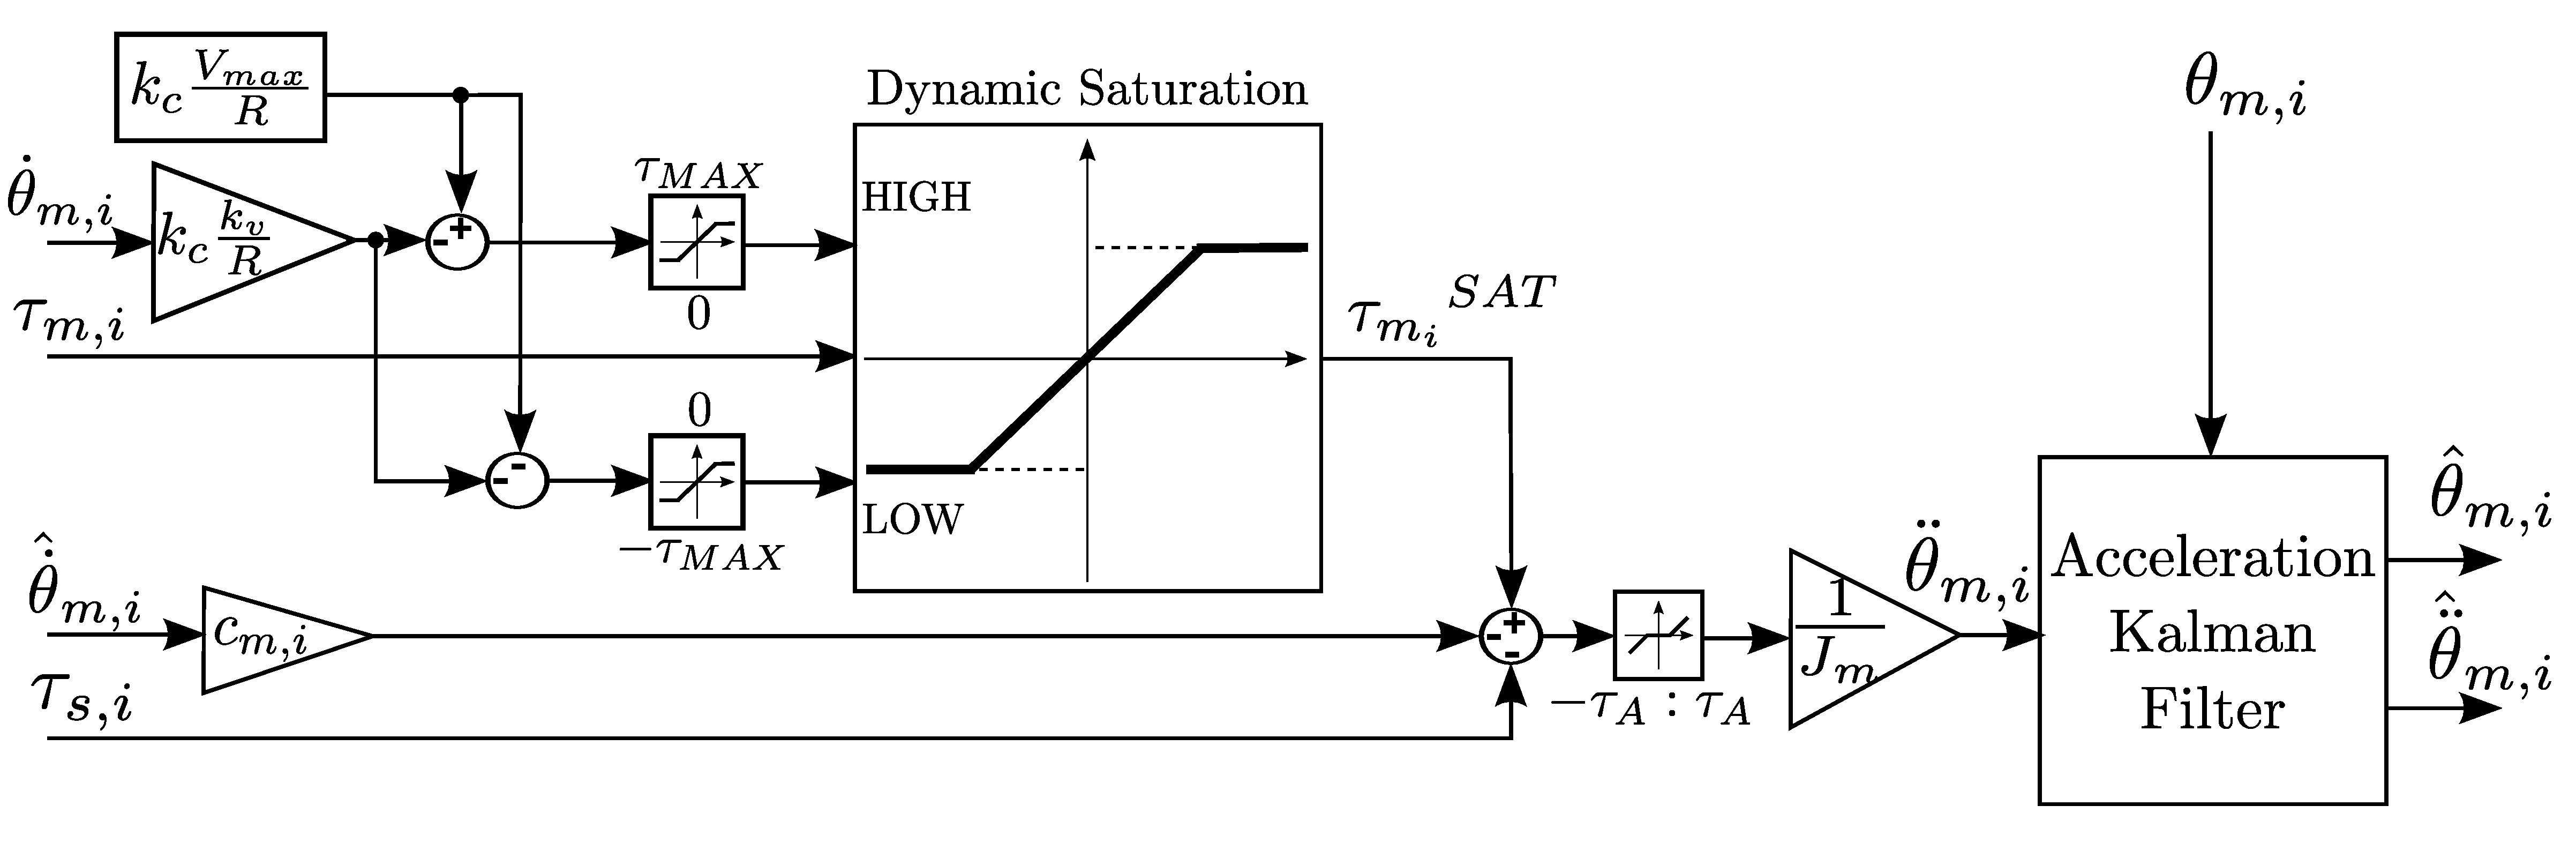
\includegraphics[width=1.0\columnwidth]{DynamicSaturation}
	\def\svgwidth{2.15\columnwidth}
	\begin{footnotesize}
		\input{imgRevised/acceleration_estimation_schema.pdf_tex}
	\end{footnotesize}
	\caption{Estimation scheme of the acceleration from torque measurement. The left side of the scheme models the motor dynamics and it considers saturation effects. The right side shows the implementation scheme of the observer.}
	\label{fig:acc_estimation}
\end{figure*}
%
%While $\tau_{s,i}$ is directly measured by the joint torque sensor  and $\tau_{m,i}$ is derived from motor command,
%an optimum Kalman observer has been used to estimate the acceleration term $\ddot{\theta}_{m,i}$
%from direct position measurements.
%

The model can be expressed in the state variable form as follows:
%

\begin{equation}
\left \{
\begin{aligned}
\vect{\dot{x}}=\vectm{A}\vect{x} + \vectmm{\Gamma}\vect{d} \\
\vect{y}=\vectm{C}\vect{x}
\end{aligned}
\right .
\end{equation}
%
where
%
\begin{equation}
\begin{aligned}
\vects{x}=\vectlong{ {\theta_{m,i}} \\ \dot{\theta}_{m,i} \\ \ddot{\theta}_{m,i}}
\vectm{A}=\mat{0 & 1 & 0  \\
	0 & 0 & 1 \\
	0 & 0 & 0 }
\vectmm{\Gamma}=\vectlong{ 0 \\ 0 \\ 1}
\vectm{C}=\mat{1 & 0 & 0  \\
	0 & 0 & 1} 
\end{aligned}
\end{equation}
%
and $\vect{d}$ is the process noise.

The observer can be formulated as:
%
\begin{equation}
\vects{\dot{\hat{x}}}=\vectm{A}\vects{\hat{x}}+\vectm{L}(\vects{y}-\vectm{C}\vects{\hat{x}})
\end{equation}
%
where L is the gain matrix of the observer. A scheme of the observer is depicted in figure \ref{fig:acc_estimation}. 
%
%\begin{figure}[htb]
%	\centering
%	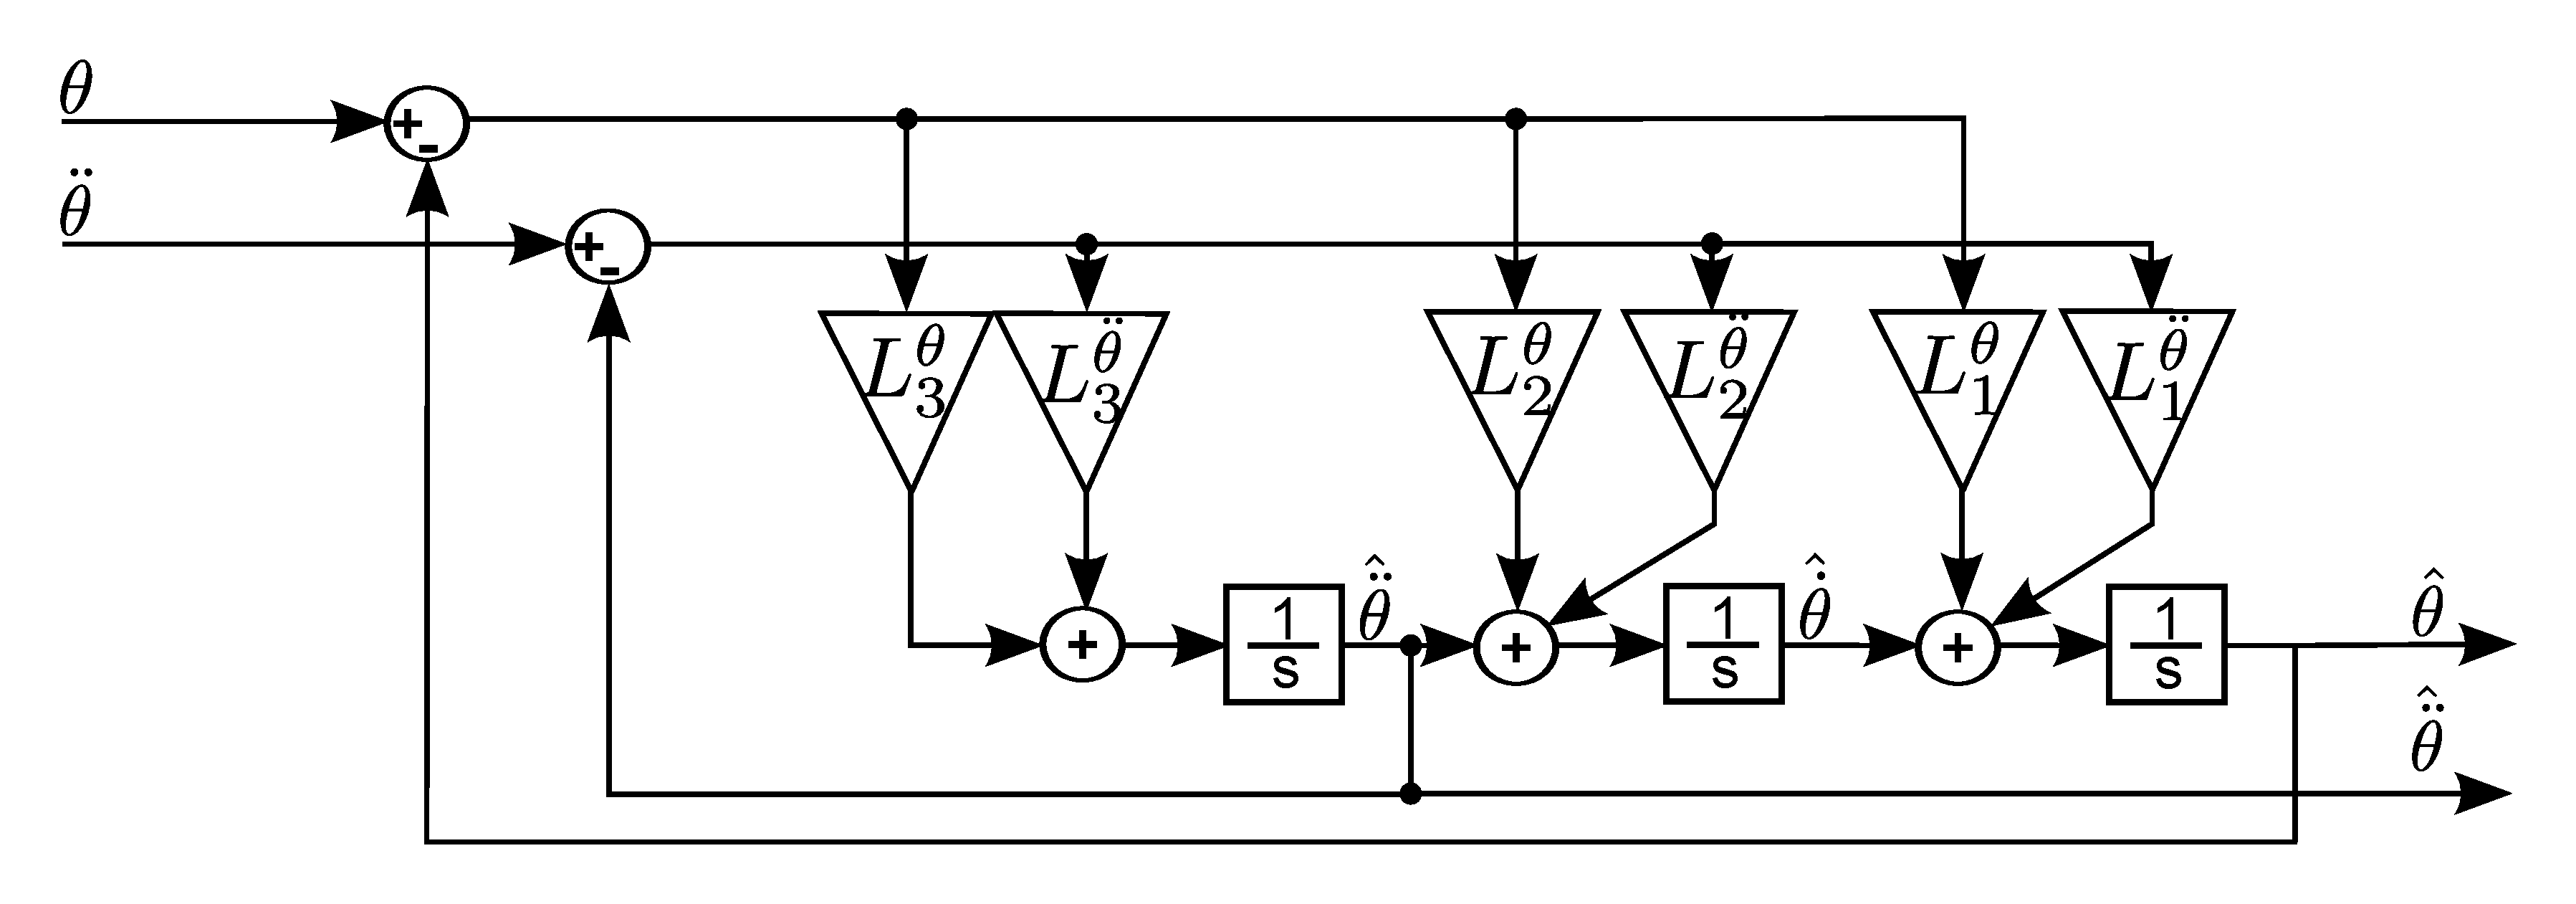
\includegraphics[width=1.0\columnwidth]{aKalmanFilter}
%	\caption{Block diagram of the acceleration observer}
%	\label{fig:block_acc_observer}
%\end{figure}

The gain $L$ was found resolving the problem of a Kalman optimum observer based on the experimental covariance data of measurement and process noise. Measurement noise was derived from motor encoder ${\theta}_{m,i}$ measurements, that mainly takes into account the encoder quantization and motor acceleration $\ddot{\theta}_{m,i}$ estimation through \eqref{tau_acc}, thanks to the available torque measurement.
%The process noise was estimated based on motor command experimental data, taking into account ripple and noise on torque generation.

%optimum observer Lueberger where the gain L has been tuned based on experimentally measured covariances on $\theta_m$ and R measurement noise,  process disturance 
As an example, the comparison between the real-time estimated acceleration (gray dotted line) and the off-line calculated acceleration (black solid line) for the first two joints is shown in figure \ref{fig:acceleration_validation}.
%
\begin{figure}[htb]
	\centering
%	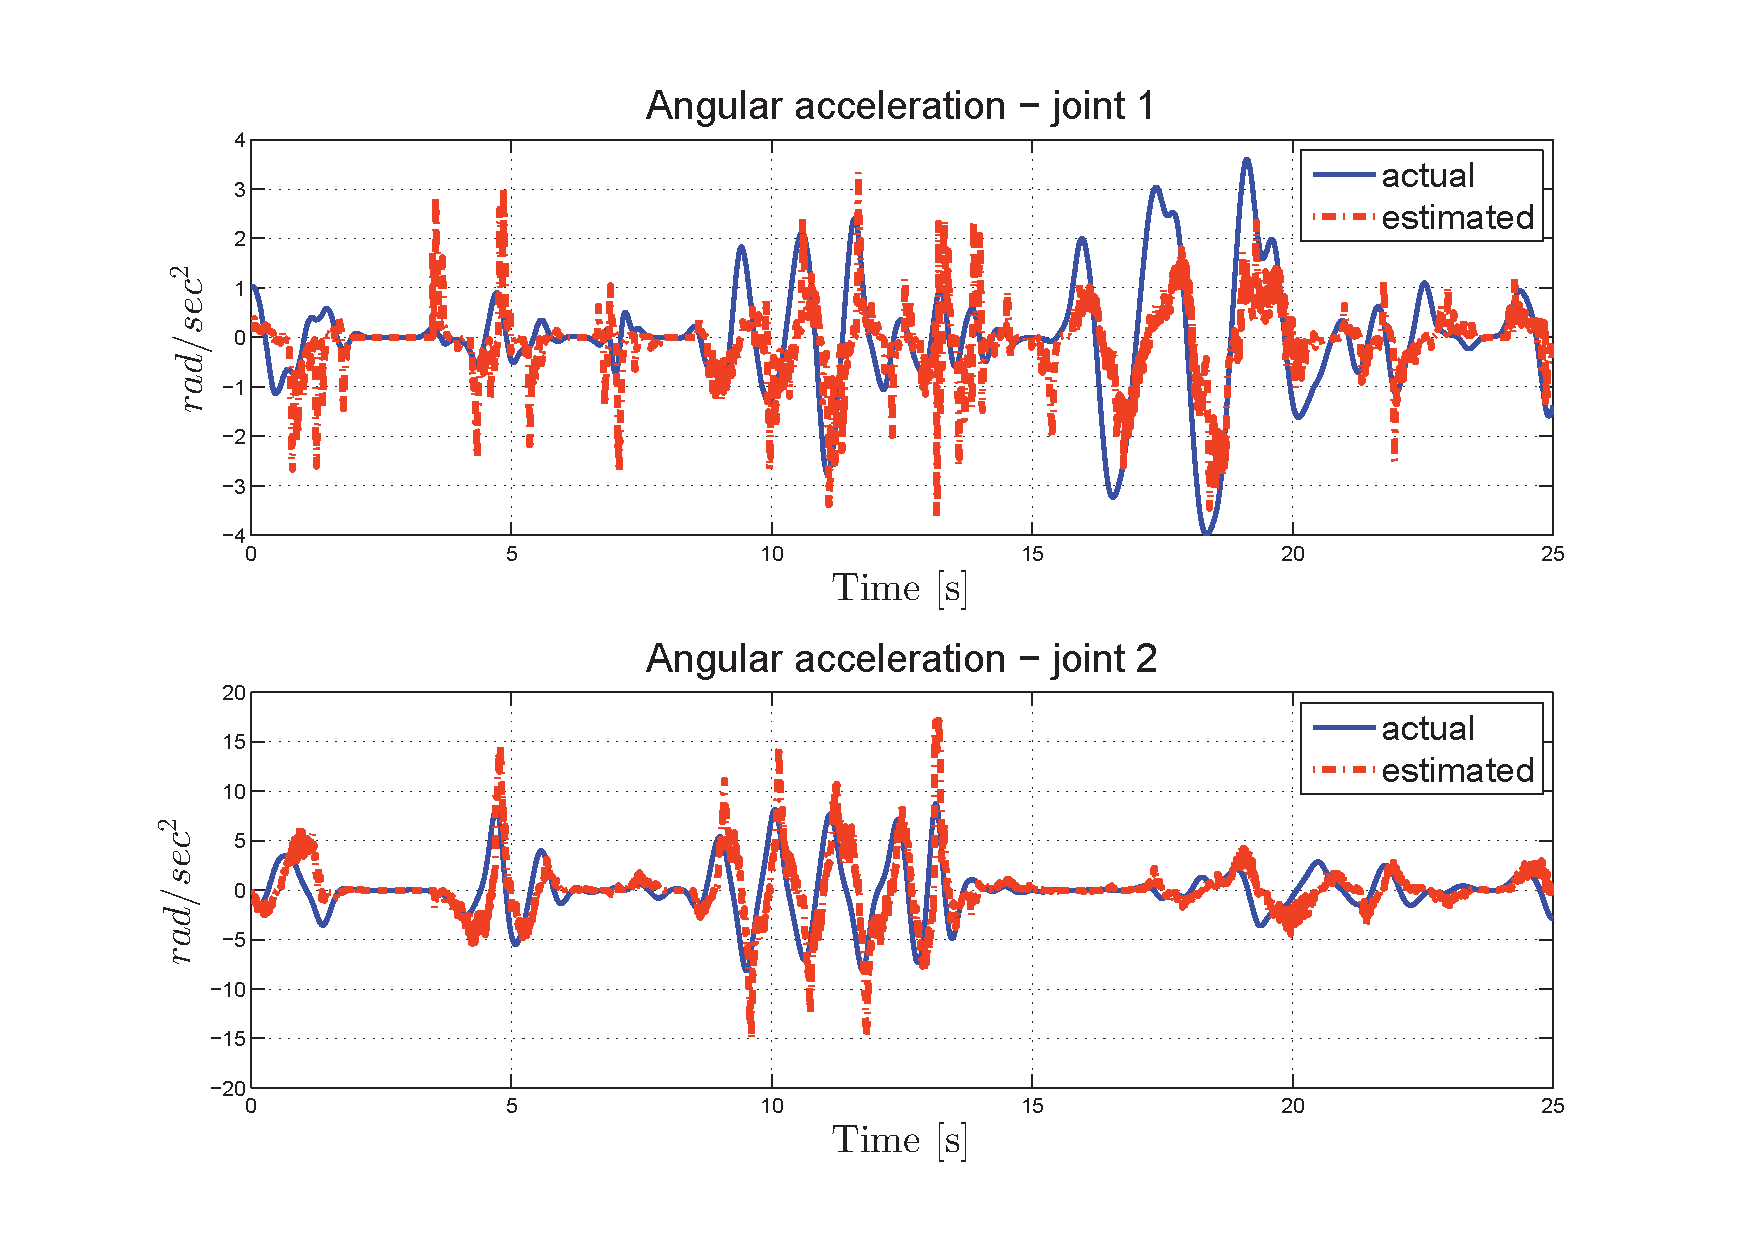
\includegraphics[width=1.0\columnwidth]{a1_a2_vs_ak1_ak2.pdf}
	\def\svgwidth{1\columnwidth}
	\begin{footnotesize}
		\input{imgRevised/acceleration_estimation.pdf_tex}
	\end{footnotesize}
	\caption{Comparison between the estimated (gray dashed line) and actual (solid black line) joint acceleration (joint 1 and 2 are chosen for reference only and similar results was obtained for all the joints). }
	\label{fig:acceleration_validation}
\end{figure}

%%%%%%%%%%%%%%%%%%%%%%%%%%%%%%%%%%%%%%%%%%%%%%%%%%%%%%%%%%%%%%%%%%%%%%%%%%%%%%%%%%%%%%%%%%%%%%%%%%%%%%%%%%%%%%%%%%%%
%%%%%%%%%%%%%%%%%%%%%%%%%%%%%%%%%%%%%%%%%%%%%%%%%%%%%%%%%%%%%%%%%%%%%%%%%%%%%%%%%%%%%%%%%%%%%%%%%%%%%%%%%%%%%%%%%%%%

\subsubsection{Dynamics compensation} \label{Dynamics compensation}

% Spiegare da dove viene fuori la storia della compensazione, dato che taul non è osservabile e che per imporre il meglio possible la taul mediante taum c'è bisogno di compensare\hl{TO DO}
As reported by equation (\ref{eq:extraForces}), the torques measured by joint sensors are due to the human force and any load applied on the links ($\vects{F_l}$). To have a good estimation of human forces by torque sensors, it is necessary to remove from torque measurements the gravity and dynamics loads applied to the links. The gravity contribution  depends only on the pose of the exoskeleton and it can be calculated by the position signals provided by the motor encoders. The gravitational term is already compensated in feed-forward by the term $\hat{\vectm{G}}(\vectm{D}\vects{\hat{\uptheta}_m})$ in $\vects{\tau_{m}}$,
except for the term $\vects{\delta} \vect{g}$.
On the other side, the dynamics contribution depends both on the pose and the acceleration and velocity of the links, which are not directly provided by any sensor, but are provided in first approximation as $\vectm{D} \vects{\hat{\ddot{\uptheta}}_m}$  by the observer described in section \ref{acc_observer}.

The dynamic torques due to the link inertias and measured by the joint torque sensors can be so estimated as the sum of the inertial contribution and the Coriolis effect:

\begin{equation}
\vects{\hat{\uptau}_{\text{dyn}}}  \eqsim \hat{\vectm{M}}(\vectm{D} \vects{\uptheta_m}) \vectm{D} \vects{\ddot{\uptheta}_m}+\hat{\vectm{C}}(\vectm{D} \vects{\uptheta_m},\vectm{D} \vects{\dot{\uptheta}_m})\vectm{D} \vects{\dot{\uptheta}_m}
\end{equation}

where matrices $\hat{\vectm{M}}$ and $\hat{\vectm{C}}$ are calculated taking into account for each joint the inertia of the parts supported by the torque sensor, discarding the inertia of the actuator of the joint.

The estimated dynamic torques are then used to compensate the dynamic effects of the link: the compensation torques $\alpha \vects{\hat{\uptau}_{\text{dyn}}} $, with $0<\alpha<1$, are a percentage of the estimated torques $\vects{\hat{\uptau}_{\text{dyn}}} $. The compensation torques are added to the desired torques $\vects{\uptau_s^D}$ as input to the state feedback controller and feed-back with the estimated torque $\vects{\hat{\uptau}_s}$. 